% autosam.tex
% Annotated sample file for the preparation of LaTeX files
% for the final versions of papers submitted to or accepted for 
% publication in AUTOMATICA.

% See also the Information for Authors.

% Make sure that the zip file that you send contains all the 
% files, including the files for the figures and the bib file.

% Output produced with the elsart style file does not imitate the
% AUTOMATICA style. The style file is generic for all Elsevier
% journals and the output is laid out for easy copy editing. The
% final document is produced from the source file in the
% AUTOMATICA style at Elsevier.

% You may use the style file autart.cls to obtain a two-column 
% document (see below) that more or less imitates the printed 
% Automatica style. This may helpful to improve the formatting 
% of the equations, tables and figures, and also serves to check 
% whether the paper satisfies the length requirements.

% Please note: Authors must not create their own macros.

% For further information regarding the preparation of LaTeX files 
% for Elsevier, please refer to the "Full Instructions to Authors" 
% from Elsevier's anonymous ftp server on ftp.elsevier.nl in the
% directory pub/styles, or from the internet (CTAN sites) on
% ftp.shsu.edu, ftp.dante.de and ftp.tex.ac.uk in the directory
% tex-archive/macros/latex/contrib/supported/elsevier.


%\documentclass{elsart}               % The use of LaTeX2e is preferred.

\documentclass[twocolumn]{autart}    % Enable this line and disable the 
                                     % preceding line to obtain a two-column 
                                     % document whose style resembles the
                                     % printed Automatica style.


\usepackage{graphicx}          % Include this line if your 
                               % document contains figures,
%\usepackage[dvips]{epsfig}    % or this line, depending on which
                               % you prefer.
\usepackage{amsmath,amssymb,amstext,amsfonts,lipsum,subfigure,bm,dsfont,epsfig,esint,stfloats,graphicx}
\usepackage{cuted}%%\stripsep-3pt
\stripsep -3pt plus 3pt minus 2pt
\usepackage{multicol}


\begin{document}

\begin{frontmatter}
%\runtitle{Insert a suggested running title}  % Running title for regular 
                                              % papers but only if the title  
                                              % is over 5 words. Running title 
                                              % is not shown in output.

\title{In Catilinam IV\thanksref{footnoteinfo}} % Title, preferably not more 
                                                % than 10 words.

\thanks[footnoteinfo]{This paper was not presented at any IFAC 
meeting. Corresponding author M.~T.~Cicero. Tel. +XXXIX-VI-mmmxxi. 
Fax +XXXIX-VI-mmmxxv.}

\author[Paestum]{Marcus Tullius Cicero}\ead{cicero@senate.ir},    % Add the 
\author[Rome]{Julius Caesar}\ead{julius@caesar.ir},               % e-mail address 
\author[Baiae]{Publius Maro Vergilius}\ead{vergilius@culture.ir}  % (ead) as shown

\address[Paestum]{Buckingham Palace, Paestum}  % Please supply                                              
\address[Rome]{Senate House, Rome}             % full addresses
\address[Baiae]{The White House, Baiae}        % here.

          
\begin{keyword}                           % Five to ten keywords,  
Cicero; Catiline; orations.               % chosen from the IFAC 
\end{keyword}                             % keyword list or with the 
                                          % help of the Automatica 
                                          % keyword wizard


\begin{abstract}                          % Abstract of not more than 200 words.
Cum M.~Cicero consul Nonis Decembribus senatum in aede Iovis 
Statoris consuleret, quid de iis coniurationis Catilinae sociis 
fieri placeret, qui in custodiam traditi essent, factum est, ut 
duae potissimum sententiae proponerentur, una D.~Silani consulis 
designati, qui morte multandos illos censebat, altera C.~Caesaris, 
qui illos publicatis bonis per municipia Italiae distribuendos 
ac vinculis sempiternis tenendos existimabat.
\end{abstract}

\end{frontmatter}

\section{Introduction}
Video, patres conscripti, in me omnium vestrum ora atque oculos esse 
conversos, video vos non solunn de vestro ac rei publicae, verum 
etiam, si id depulsum sit, de meo periculo esse sollicitos. Est mihi 
iucunda in malis et grata in dolore vestra erga me voluntas, sed eam, 
per deos inmortales, deponite atque obliti salutis meae de vobis ac 
de vestris liberis cogitate. Mihi si haec condicio consulatus data 
est, ut omnis acerbitates, onunis dolores cruciatusque perferrem, 
feram non solum fortiter, verum etiam lubenter, dum modo meis 
laboribus vobis populoque Romano dignitas salusque pariatur.

A novel LOI(linear operator Inequality) approach have been proposed by Peet

A new method converting from DDE to PIE and the method converting from NDS to PIE 
have been proposed by Representation of Networks and Systems with Delay:DDEs, DDFs, 
ODE-PDEs and PIEs,comparing with the method used by Delay-Dependent Stability for 
Load Frequency Control System via Linear Operator Inequality, the new method can 
convert not only multiple time-delay system but also the nuetral delay system(NDS) 
even the neutral system with Integral term.

In this article,we consider the stability of the neutral system by using the new method 
proposed by Peet.




% OR

%\begin{figure}
%\begin{center}
%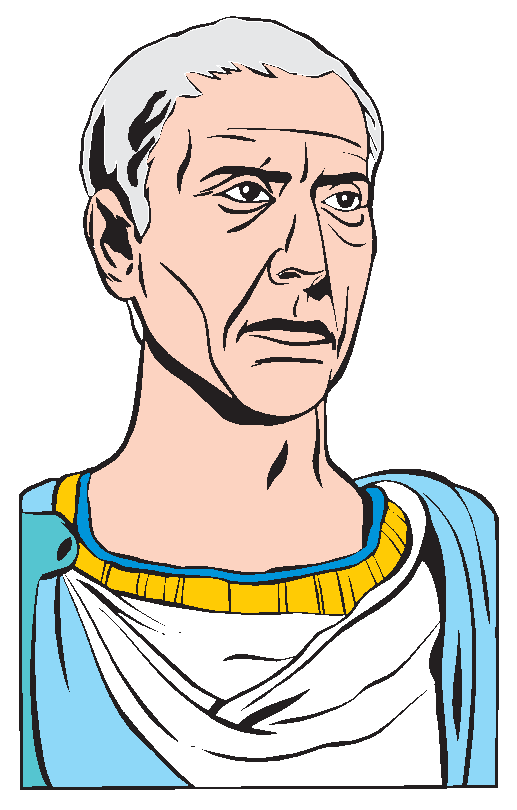
\epsfig{file=jcaesar,width=7cm}
%\caption{Gaius Julius Caesar, 100--44 B.C.}
%\label{fig1}
%\end{center}
%\end{figure}

\subsection{A subsection}
Marcus Tullius Cicero, 106--43 B.C. was a Roman statesman, orator, 
and philosopher.  A major figure in the last years of the Republic, 
he is best known for his orations against Catiline\footnote{
This footnote should be very brief.}
and for his mastery of Latin prose \cite{Heritage:92}. He was a 
contemporary of Julius Caesar (Fig.~\ref{fig1}).

\section{Problem formulation and preliminaries}
Consider a neutral system described by the following equation:
%See \cite{Abl:56}, \cite{AbTaRu:54}, \cite{Keo:58} and 
%\cite{Pow:85}.
\begin{equation} \label{e1}
    \begin{aligned}
        \dot{x}(t) = A_{0}x(t) & +B_{1}w(t)+B_{2}u(t) \\ 
        &+\sum_{i=1}^{K}[A_{i}x(t-\tau_{i})+B_{1i}w(t-\tau_{i}) \\ 
        &+B_{2i}u(t-\tau_{i})+E_{i}\dot{x}(t-\tau_{i})]
    \end{aligned}
\end{equation}
If we do not consider the interfere $w(t)$
\begin{equation} \label{e1}
    \begin{aligned}
    \dot{x}(t) = A_{0}x(t)+B_{2}u(t) & +\sum_{i=1}^{K}[A_{i}x(t-\tau_{i})\\
    & +B_{2i}u(t-\tau_{i})+E_{i}\dot{x}(t-\tau_{i})]
    \end{aligned}
\end{equation}
If we also do not consider the output $y(t)$,we can convert Equation (2) to standard NDS(neutral delay system) form Equation (3) by the Equation (4)
\begin{equation}
    \begin{aligned}
        \begin{bmatrix}
            \dot{x}(t) \\
            z(t) \\
            y(t) 
        \end{bmatrix} & = \begin{bmatrix}
            A_{0} & 0 & B_{2}\\
            0 & 0 & 0\\
            0 & 0 & 0
        \end{bmatrix}\begin{bmatrix}
            x(t) \\
            w(t) \\
            u(t) 
        \end{bmatrix} \\ 
        &+ \sum_{i=1}^{K}\begin{bmatrix}
            A_{i} & 0 & B_{2i} & E_{i}\\
            0 & 0 & 0 & 0\\
            0 & 0 & 0 & 0
        \end{bmatrix} \begin{bmatrix}
            x(t-\tau_{i}) \\
            w(t-\tau_{i}) \\
            u(t-\tau_{i}) \\
            \dot{x}(t-\tau_{i})
        \end{bmatrix}.\label{eq}
    \end{aligned}
\end{equation}

And then cite Representation of Networks and Systems with Delay:DDEs, DDFs, ODE-PDEs and PIEs ,we can convert standard NDS form Equation (3) to DDF(Differential Difference Equations) form Eqution (7) by Eqution (4)


%Conversion Formula from NDS to DDF LEMMA2
\begin{figure*}[hb] %hb代表放在文章底部,%ht为放在文章顶部 
    \flushleft
    {\noindent}	 \rule[-10pt]{17.5cm}{0.05em}\\
    \vspace{1.5em}
    \text{Conversion Formula from NDS to DDF:}
    %\centering
    \begin{equation}
        \begin{aligned}
            D_{rvi} &= 
            \begin{bmatrix}
                0 & 0 & 0 \\
                0 & 0 & 0 \\
                0 & 0 & 0 \\
                I & 0 & 0
            \end{bmatrix}       ,    & [C_{ri} \space B_{r1i} \space B_{r2i}] &= 
                                        \begin{bmatrix}
                                            I_{n} & 0 & 0 \\
                                            0 & I_{m} & 0 \\
                                            0 & 0 & I_{p} \\
                                            A_{0} & 0 & B_{2}
                                            \end{bmatrix}  ,                           & I_{n+q+r}&= 
                                                                                        \begin{bmatrix}
                                                                                            B_{v} \\
                                                                                            D_{1v} \\
                                                                                            D_{2v} 
                                                                                        \end{bmatrix}\ \\
            C_{vi} &= 
            \begin{bmatrix}
                A_{i} & 0 & B_{2i} & E_{i} \\
                0 & 0 & 0 & 0\\
                0 & 0 & 0 & 0\\
                0 & 0 & 0 & 0
            \end{bmatrix}  ,              & C_{vdi}(s) &= 0 
        \end{aligned}
    \end{equation}
\end{figure*}

%Conversion Formula from ODE-PDE to DDF to PIE(1) LEMMA4
\begin{figure*}[ht] %hb代表放在文章底部,%ht为放在文章顶部 
    \flushleft
    \text{Conversion Formula from ODE-PDE to DDF to PIE:}
\begin{equation}
    \begin{aligned}
        &\mathcal{A} = \mathcal{P} 
            \begin{bmatrix}
                A_{0} & A \\
                0 & \{I_{\tau},0,0\} 
            \end{bmatrix} ,\quad &\mathcal{T} = \mathcal{P} 
            \begin{bmatrix}
                I & 0 \\
                T_{0} & \{0,T_{a},T_{b}\} 
            \end{bmatrix},\quad &\mathcal{B}_{T_{1}} = \mathcal{P} 
            \begin{bmatrix}
                0 & \varnothing \\
                T_{1} & \{\varnothing\} 
            \end{bmatrix} ,\quad &\mathcal{B}_{T_{2}} = \mathcal{P} 
            \begin{bmatrix}
                0 & \varnothing \\
                T_{2} & \{\varnothing\} 
            \end{bmatrix},\\
        &\mathcal{B}_{1} = \mathcal{P} 
        \begin{bmatrix}
            \bold{B_{1}} & \varnothing \\
            0 & \{\varnothing\} 
        \end{bmatrix},\quad &\mathcal{B}_{2} = \mathcal{P} 
        \begin{bmatrix}
            \bold{B_{2}} & \varnothing \\
            0 & \{\varnothing\} 
        \end{bmatrix},\quad &\mathcal{C}_{1} = \mathcal{P} 
        \begin{bmatrix}
            \bold{C_{10}} & \bold{C_{11}} \\
            \varnothing & \{\varnothing\} 
        \end{bmatrix}, \quad &\mathcal{C}_{2} = \mathcal{P} 
        \begin{bmatrix}
            \bold{C_{20}} & \bold{C_{21}} \\
            \varnothing & \{\varnothing\} 
        \end{bmatrix}
    \end{aligned}
\end{equation}
\vspace{1.5em}
{\noindent}	 \rule[-10pt]{17.5cm}{0.05em}\\
\end{figure*}

%ODE-PDE to DDF to PIE(2)
\begin{figure*}[ht] %hb代表放在文章底部,%ht为放在文章顶部 
    \flushleft
    \begin{equation}
        \begin{aligned}
            &\hat{C}_{vi} = C_{vi},    \quad \quad \quad \quad  D_{I} = 
                                            \begin{bmatrix}
                                                (I-\sum_{i=1}^{K}C_{vi}D_{rvi})^{-1} & 0 & 0 \\
                                                0 & 0 & 0 \\
                                                0 & 0 & I
                                            \end{bmatrix}  ,            \\
            &C_{Ii} = -D_{I}C_{vi} = \begin{bmatrix}
                -(I-\sum_{i=1}^{K}E_{i})^{-1}A_{i} & 0 & -(I-\sum_{i=1}^{K}E_{i})^{-1}B_{2i} & -(I-\sum_{i=1}^{K}E_{i})^{-1}E_{i} \\
                0 & 0 & 0 & 0\\
                0 & 0 & 0 & 0\\
                0 & 0 & 0 & 0
                \end{bmatrix}
                ,           \\   
            &[T_{0} \quad T_{1} \quad T_{2}] = \begin{bmatrix}
                C_{r1}+D_{rv1}C_{vx} & C_{r1}+D_{rv1}D_{vw}  & C_{r1}+D_{rv1}D_{vu}  \\
                C_{r2}+D_{rv2}C_{vx} & C_{r2}+D_{rv2}D_{vw}  & C_{r2}+D_{rv2}D_{vu}  \\
                \vdots & \vdots & \vdots \\
                C_{rK}+D_{rvK}C_{vx} & C_{rK}+D_{rvK}D_{vw}  & C_{rK}+D_{rvK}D_{vu}   
            \end{bmatrix},\\
            &C_{r1}+D_{rv1}C_{vx} = 
            \begin{bmatrix}
            I_{n}    \\
            0        \\
            A_{0}+(I-\sum_{i=1}^{K}E_{i})^{-1}(\sum_{i=1}^{K}(A_{i}+E_{i}A_{0})
            \end{bmatrix},\\
            &[C_{vx} \quad D_{vw} \quad D_{vu}] = \begin{bmatrix}
                (I-\sum_{i=1}^{K}E_{i})^{-1}(\sum_{i=1}^{K}(A_{i}+E_{i}A_{0})  & (I-\sum_{i=1}^{K}E_{i})^{-1}(E_{i}B_{1}) & (I-\sum_{i=1}^{K}E_{i})^{-1}(E_{i}B_{2}) \\
                0 &  0 & 0\\
                0 &  0 & 0
            \end{bmatrix},\\
            &T_{a}(s,\theta) = 
            \begin{bmatrix}
                D_{rv1}C_{I1} & D_{rv1}C_{I2} & \dots & D_{rv1}C_{IK}   \\
                D_{rv2}C_{I1} & D_{rv2}C_{I2} & \dots & D_{rv2}C_{IK}        \\
                \vdots & \vdots & \vdots & \vdots\\ 
                D_{rvK}C_{I1} & D_{rvK}C_{I2} & \dots & D_{rvK}C_{IK}
            \end{bmatrix},\\
            &D_{rv1}C_{I1} = 
            \begin{bmatrix}
                0 & 0 & 0 & 0   \\
                0 & 0 & 0 & 0          \\
                0 & 0 & 0 & 0  \\ 
                -(I-\sum_{i=1}^{K}E_{i})^{-1}A_{1} & 0 & -(I-\sum_{i=1}^{K}E_{i})^{-1}B_{21} & -(I-\sum_{i=1}^{K}E_{i})^{-1}E_{1}
            \end{bmatrix},\\
            &T_{b}(s,\theta) = -I_{\sum_{i}p_{i}} + T_{a}(s,\theta) = \begin{bmatrix}
                                                                    -I & 0 & 0 & 0   \\
                                                                    0 & -I & 0 & 0          \\
                                                                    0 & 0 & -I & 0  \\ 
                                                                    -(I-\sum_{i=1}^{K}E_{i})^{-1}A_{1} & 0 & -(I-\sum_{i=1}^{K}E_{i})^{-1}B_{21} & -I-(I-\sum_{i=1}^{K}E_{i})^{-1}E_{1}
                                                                \end{bmatrix},\\
            &I_{\tau} = 
            \begin{bmatrix}
            \frac{1}{\tau_{1}}I_{p1} & 0 & 0 & 0   \\
            0 & \frac{1}{\tau_{2}}I_{p2} & 0 & 0          \\
            0 & 0 &\ddots & 0  \\ 
            0 & 0 & 0 & \frac{1}{\tau_{K}}I_{pK}
            \end{bmatrix},    \quad \begin{bmatrix}
                                                        A \\
                                                        C_{11} \\
                                                        C_{21} 
                                                    \end{bmatrix}= 
                                                    \begin{bmatrix}
                                                        B_{v} \\
                                                        D_{1v} \\
                                                        D_{2v} 
                                                    \end{bmatrix}[C_{I1} \dots C_{IK}],   \quad\begin{bmatrix}
                                                        \bold{A_{0}} & \bold{B_{1}} & \bold{B_{2}} \\
                                                        \bold{C_{10}} & \bold{D_{11}} & \bold{D_{12}} \\
                                                        \bold{C_{20}} & \bold{D_{21}} & \bold{D_{22}} 
                                                    \end{bmatrix} = 
                                                    \begin{bmatrix}
                                                        A_{0} & B_{1} & B_{2} \\
                                                        C_{10} & D_{11} & D_{12} \\
                                                        C_{20} & D_{21} & D_{22}
                                                    \end{bmatrix}[C_{vx} \quad D_{vw} \quad D_{vu}],\\
\end{aligned}
    \end{equation}
    \vspace{1.5em}
{\noindent}	 \rule[-10pt]{17.5cm}{0.05em}\\
\end{figure*}

then we get the standard DDF form
\begin{equation}
    \begin{aligned}
        \begin{bmatrix}
            \dot{x}(t) \\
            z(t) \\
            y(t) \\
            r_{i}(t)
        \end{bmatrix} & = \begin{bmatrix}
            A_{0} & 0 & B_{2}\\
            0 & 0 & 0\\
            0 & 0 & 0\\
            C_{ri} & B_{r1i} & B_{r2i}
        \end{bmatrix}\begin{bmatrix}
            x(t) \\
            w(t) \\
            u(t) 
        \end{bmatrix} 
        +  \begin{bmatrix}
            B_{v} \\
            D_{1v} \\
            D_{2v} \\
            D_{rvi}
        \end{bmatrix}v(t)\\
        v(t) &= \sum_{i = 1}^{K}C_{vi}r(t-\tau_{i})
    \end{aligned}
\end{equation}

And then we try to cite Representation of Networks and Systems with Delay:DDEs, DDFs, ODE-PDEs and PIEs convert standard DDF form Equation (7) to PIE from Equation (8) 
\begin{equation}
    \begin{aligned}
        \setlength{\arraycolsep}{0.9pt}
        \mathcal{T}\dot{\bold{x}}+\mathcal{B}_{T_{2}}\dot{u} = \mathcal{A}\bold{x}+\mathcal{B}_{2}u
    \end{aligned}
\end{equation}
If we introduce the controller,
\begin{equation}
    \begin{aligned}
        \setlength{\arraycolsep}{0.9pt}
        u(t) = K\bold{x(t)}
    \end{aligned}
\end{equation}
\begin{equation}
    \begin{aligned}
        \setlength{\arraycolsep}{0.9pt}
        \bold{x(t)} := \begin{bmatrix}
            x(t) \\
            \Phi(t,.)
        \end{bmatrix}\nonumber
    \end{aligned}
\end{equation}
then we got the standard PIE form 
\begin{equation}
    \begin{aligned}
        \setlength{\arraycolsep}{0.9pt}
        \mathcal{T}\dot{\bold{x}}+\mathcal{B}_{T_{2}}K\dot{x} = \mathcal{A}\bold{x}+\mathcal{B}_{2}Kx
    \end{aligned}
\end{equation}
Next we will do some variable substitution
\begin{equation}
    \begin{aligned}
        \setlength{\arraycolsep}{0.9pt}
        \mathcal{T}' = \mathcal{T}+\mathcal{B}_{T_{2}}K
    \end{aligned}
\end{equation}

\begin{equation}
    \begin{aligned}
        \setlength{\arraycolsep}{0.9pt}
        \mathcal{A}' = \mathcal{A}+\mathcal{B}_{2}K
    \end{aligned}
\end{equation}
then we got a more concise PIE form
\begin{equation}
    \begin{aligned}
        \setlength{\arraycolsep}{0.9pt}
        \mathcal{T}'\dot{\bold{x}} = \mathcal{A}'\bold{x}
    \end{aligned}
\end{equation}
remark?
It should be noticed that is the difference between $\bold{x}$ and $x$.
The reason why $\bold{x}$ terms and $x$ terms can be added up is that there is no difference
for the operator $\mathcal{B}_{T_{2}}$ to dual with $\bold{x}$ and $x$.


\section{Stability Analysis}
Cite Delay-Dependent Stability for Load FrequencyControl System via Linear Operator Inequality 

\begin{thm}
    \begin{equation}
        \begin{aligned}
            \setlength{\arraycolsep}{0.9pt}
            \mathcal{T}'^{*}\mathcal{H}\mathcal{A}'+\mathcal{A}'^{*}\mathcal{H}\mathcal{T}' \textless 0
        \end{aligned}
    \end{equation}
\end{thm}

Proof:\\
L-K funtional 
\begin{equation}
    \begin{aligned}
        \setlength{\arraycolsep}{0.9pt}
        V(\bold{x}) &= <\mathcal{T}\bold{x},\mathcal{H}\mathcal{A}\bold{x}>_{Z} 
    \end{aligned}
\end{equation}
\begin{equation}
    \begin{aligned}
        \setlength{\arraycolsep}{0.9pt}
        \dot{V}(\bold{x}) &= <\mathcal{T}'\bold{x},\mathcal{H}\mathcal{T}'\bold{x}>_{Z} + <\mathcal{A}'\bold{x},\mathcal{H}\mathcal{T}'\bold{x}>_{Z} \\ &=<\bold{x},(\mathcal{T}'^{*}\mathcal{H}\mathcal{A}'+\mathcal{A}'^{*}\mathcal{H}\mathcal{T}')\bold{x}>_{Z}  
    \end{aligned}
\end{equation}
remark?
The procedures for calculating the delay margin are provided as follows.?






\section{Case Studies Using \emph{PIETOOLS2022a}}

\begin{equation}
    \begin{aligned}
        \begin{bmatrix}
            \dot{x}(t) \\
            z(t) \\
            y(t) 
        \end{bmatrix} & = \begin{bmatrix}
            A_{0} & 0 & 0\\
            0 & 0 & 0\\
            0 & 0 & 0
        \end{bmatrix}\begin{bmatrix}
            x(t) \\
            w(t) \\
            u(t) 
        \end{bmatrix} \\ 
        &+ \begin{bmatrix}
            A_{1} & 0 &0 & E_{1}\\
            0 & 0 & 0 & 0\\
            0 & 0 & 0 & 0
        \end{bmatrix} \begin{bmatrix}
            x(t-\tau_{1}) \\
            w(t-\tau_{1}) \\
            u(t-\tau_{1}) \\
            \dot{x}(t-\tau_{1})
        \end{bmatrix}\\
        &+ \begin{bmatrix}
            A_{2} & 0 &0 & E_{2}\\
            0 & 0 & 0 & 0\\
            0 & 0 & 0 & 0
        \end{bmatrix} \begin{bmatrix}
            x(t-\tau_{2}) \\
            w(t-\tau_{2}) \\
            u(t-\tau_{2}) \\
            \dot{x}(t-\tau_{2})
        \end{bmatrix}.\label{eq}
    \end{aligned}
\end{equation}



\begin{equation}
    \begin{aligned}
        &A_{0} =  \begin{bmatrix}
            -2 & 1\\
            0 & -1\\
        \end{bmatrix}
        &A_{1} =  \begin{bmatrix}
            0 & 0.3\\
            -0.3 & 0
        \end{bmatrix}\\
        &A_{2} =  \begin{bmatrix}
            0.1 & 0.05\\
            -0.05 & 0.1
        \end{bmatrix}
        &E_{1} =  \begin{bmatrix}
            0 & -0.1\\
            -0.1 & 0\\
        \end{bmatrix}\\
        &E_{2} =  \begin{bmatrix}
            0.05 & 0\\
            -0 & 0.05
        \end{bmatrix}\\
        &\tau_{1} =  2.262, \quad \tau_{2} =  0.5
    \end{aligned}
\end{equation}



need Tables!!



\section{Conclusion}
cite Delay-Dependent Stability for Load FrequencyControl System via Linear Operator Inequality 
\begin{equation}
    \begin{aligned}
        \setlength{\arraycolsep}{0.9pt}
        \mathcal{T}'^{*}\mathcal{H}\mathcal{A}'+\mathcal{A}'^{*}\mathcal{H}\mathcal{T}' \textless 0
    \end{aligned}
\end{equation}
$\bold{PROOF:}$ 
\begin{equation}
    \begin{aligned}
        \setlength{\arraycolsep}{0.9pt}
        \dot{V}(\bold{x}) &= <\mathcal{T}'\bold{x},\mathcal{H}\mathcal{T}'\bold{x}>_{Z} + <\mathcal{A}'\bold{x},\mathcal{H}\mathcal{T}'\bold{x}>_{Z} \\ &=<\bold{x},(\mathcal{T}'^{*}\mathcal{H}\mathcal{A}'+\mathcal{A}'^{*}\mathcal{H}\mathcal{T}')\bold{x}>_{Z}  
    \end{aligned}
\end{equation}
\section{References}
cite Delay-Dependent Stability for Load FrequencyControl System via Linear Operator Inequality 
\begin{equation}
    \begin{aligned}
        \setlength{\arraycolsep}{0.9pt}
        \mathcal{T}'^{*}\mathcal{H}\mathcal{A}'+\mathcal{A}'^{*}\mathcal{H}\mathcal{T}' \textless 0
    \end{aligned}
\end{equation}
\begin{equation}
    \begin{aligned}
        \setlength{\arraycolsep}{0.9pt}
        \dot{V}(\bold{x}) &= <\mathcal{T}'\bold{x},\mathcal{H}\mathcal{T}'\bold{x}>_{Z} + <\mathcal{A}'\bold{x},\mathcal{H}\mathcal{T}'\bold{x}>_{Z} \\ &=<\bold{x},(\mathcal{T}'^{*}\mathcal{H}\mathcal{A}'+\mathcal{A}'^{*}\mathcal{H}\mathcal{T}')\bold{x}>_{Z}  
    \end{aligned}
\end{equation}

\section{Appendixes}
$\bold{PROOF:}$ lemma2\\
Given NDS form
\begin{equation}
    \begin{aligned}
        \begin{bmatrix}
            \dot{x}(t) \\
            z(t) \\
            y(t) 
        \end{bmatrix} & = \begin{bmatrix}
            A_{0} & 0 & B_{2}\\
            0 & 0 & 0\\
            0 & 0 & 0
        \end{bmatrix}\begin{bmatrix}
            x(t) \\
            w(t) \\
            u(t) 
        \end{bmatrix} \\ 
        &+ \sum_{i=1}^{K}\begin{bmatrix}
            A_{i} & 0 & B_{2i} & E_{i}\\
            0 & 0 & 0 & 0\\
            0 & 0 & 0 & 0
        \end{bmatrix} \begin{bmatrix}
            x(t-\tau_{i}) \\
            w(t-\tau_{i}) \\
            u(t-\tau_{i}) \\
            \dot{x}(t-\tau_{i})
        \end{bmatrix}\\
    \end{aligned}
\end{equation}
assume that
\begin{equation}
    \begin{aligned}
        v(t) &= \sum_{i = 1}^{K}C_{vi}r_{i}(t-\tau_{i})
    \end{aligned}
\end{equation}
then we get
\begin{equation}
    \begin{aligned}
        \begin{bmatrix}
            \dot{x}(t) \\
            z(t) \\
            y(t) 
        \end{bmatrix} & = \begin{bmatrix}
            A_{0} & 0 & B_{2}\\
            0 & 0 & 0\\
            0 & 0 & 0
        \end{bmatrix}\begin{bmatrix}
            x(t) \\
            w(t) \\
            u(t) 
        \end{bmatrix} + Iv(t)\\
    \end{aligned}
\end{equation}
$I$ is a identity matrix,we define
\begin{equation}
    \begin{aligned}
        I & = \begin{bmatrix}
            B_{v} \\
            D_{1v} \\
            D_{2v} 
        \end{bmatrix} \\
    \end{aligned}
\end{equation}
so that
\begin{equation}
    \begin{aligned}
        \begin{bmatrix}
            \dot{x}(t) \\
            z(t) \\
            y(t) 
        \end{bmatrix} & = \begin{bmatrix}
            A_{0} & 0 & B_{2}\\
            0 & 0 & 0\\
            0 & 0 & 0
        \end{bmatrix}\begin{bmatrix}
            x(t) \\
            w(t) \\
            u(t) 
        \end{bmatrix} + \begin{bmatrix}
            B_{v} \\
            D_{1v} \\
            D_{2v} 
        \end{bmatrix}v(t)\\
    \end{aligned}
\end{equation}

from the above eqution,we get
\begin{equation}
    \begin{aligned}
            \dot{x}(t) 
        & = \begin{bmatrix}
            A_{0} & 0 & B_{2}
        \end{bmatrix}\begin{bmatrix}
            x(t) \\
            w(t) \\
            u(t) 
        \end{bmatrix} + 
            B_{v} v(t)\\
    \end{aligned}
\end{equation}

we can see $B_{v}v(t)$ Representing the first part of $v(t)$,so we get
\begin{equation}
    \begin{aligned}
            B_{v} v(t) = \begin{bmatrix}
                I & 0 & 0
            \end{bmatrix}v(t)
    \end{aligned}
\end{equation}

define 
\begin{equation}
    \begin{aligned}
        r_{i}(t) = \begin{bmatrix}
            x(t) \\
            z(t) \\
            y(t) \\
            \dot{x}(t)
        \end{bmatrix} 
    \end{aligned}
\end{equation}


\begin{equation}
    \begin{aligned}
        r_{i}(t) &= \begin{bmatrix}
            x(t) \\
            z(t) \\
            y(t) \\
            \dot{x}(t)
        \end{bmatrix} = \begin{bmatrix}
            I & 0 & 0 \\
            0 & I & 0  \\
            0 & 0 & I  \\
            0 & 0 & 0 
        \end{bmatrix}\begin{bmatrix}
            x(t) \\
            w(t) \\
            u(t) 
        \end{bmatrix}+\begin{bmatrix}
            0 \\
            0 \\
            0 \\
            \dot{x}(t)
        \end{bmatrix}\\
        &= \begin{bmatrix}
            I & 0 & 0 \\
            0 & I & 0  \\
            0 & 0 & I  \\
            A_{0} & 0 & B_{2} 
        \end{bmatrix}\begin{bmatrix}
            x(t) \\
            w(t) \\
            u(t) 
        \end{bmatrix}+\begin{bmatrix}
            0 & 0 & 0 \\
            0 & 0 & 0\\
            0 & 0 & 0\\
            I & 0 & 0
        \end{bmatrix}v(t)
    \end{aligned}
\end{equation}

Cite [NDS to DDF] we get
\begin{equation}
    \begin{aligned}
            r_{i}(t) & = \begin{bmatrix}
            C_{ri} & B_{r1i} & B_{r2i}
        \end{bmatrix}\begin{bmatrix}
            x(t) \\
            w(t) \\
            u(t) 
        \end{bmatrix} 
        + D_{rvi}v(t)
    \end{aligned}
\end{equation}

merge eqution (27) and eqution (30),we get the standard DDF form
\begin{equation}
    \begin{aligned}
        \begin{bmatrix}
            \dot{x}(t) \\
            z(t) \\
            y(t) \\
            r_{i}(t)
        \end{bmatrix} & = \begin{bmatrix}
            A_{0} & 0 & B_{2}\\
            0 & 0 & 0\\
            0 & 0 & 0\\
            C_{ri} & B_{r1i} & B_{r2i}
        \end{bmatrix}\begin{bmatrix}
            x(t) \\
            w(t) \\
            u(t) 
        \end{bmatrix} + \begin{bmatrix}
            B_{v} \\
            D_{1v} \\
            D_{2v} \\
            D_{rvi}
        \end{bmatrix}v(t)\\
    \end{aligned}
\end{equation}


$\bold{PROOF:}$ lemma4\\

\end{document}